%%%%%%%%%%%%%%%%%%%%%%%%%%%%%%%%%%%%%%%%%
% Short Sectioned Assignment
% LaTeX Template
% Version 1.0 (5/5/12)
%
% This template has been downloaded from:
% http://www.LaTeXTemplates.com
%
% Original author:
% Frits Wenneker (http://www.howtotex.com)
%
% License:
% CC BY-NC-SA 3.0 (http://creativecommons.org/licenses/by-nc-sa/3.0/)
%
%%%%%%%%%%%%%%%%%%%%%%%%%%%%%%%%%%%%%%%%%

%----------------------------------------------------------------------------------------
%	PACKAGES AND OTHER DOCUMENT CONFIGURATIONS
%----------------------------------------------------------------------------------------

\documentclass[paper=a4, fontsize=11pt]{scrartcl} % A4 paper and 11pt font size

\usepackage[T1]{fontenc} % Use 8-bit encoding that has 256 glyphs
\usepackage{fourier} % Use the Adobe Utopia font for the document - comment this line to return to the LaTeX default
\usepackage[english]{babel} % English language/hyphenation
\usepackage{amsmath,amsfonts,amsthm} % Math packages
\usepackage[utf8]{inputenc}
\usepackage{graphicx}
\usepackage{tabularx}
\usepackage{longtable}
\usepackage{threeparttable}
\usepackage{booktabs}
\usepackage{listings}
\usepackage[numbered,autolinebreaks,useliterate]{mcode}
\usepackage{float}
\usepackage{algpseudocode}

\usepackage{lipsum} % Used for inserting dummy 'Lorem ipsum' text into the template

\usepackage{sectsty} % Allows customizing section commands
\allsectionsfont{\centering \normalfont\scshape} % Make all sections centered, the default font and small caps

\usepackage{fancyhdr} % Custom headers and footers
\pagestyle{fancyplain} % Makes all pages in the document conform to the custom headers and footers
\fancyhead{} % No page header - if you want one, create it in the same way as the footers below
\fancyfoot[L]{} % Empty left footer
\fancyfoot[C]{} % Empty center footer
\fancyfoot[R]{\thepage} % Page numbering for right footer
\renewcommand{\headrulewidth}{0pt} % Remove header underlines
\renewcommand{\footrulewidth}{0pt} % Remove footer underlines
\setlength{\headheight}{13.6pt} % Customize the height of the header

\numberwithin{equation}{section} % Number equations within sections (i.e. 1.1, 1.2, 2.1, 2.2 instead of 1, 2, 3, 4)
\numberwithin{figure}{section} % Number figures within sections (i.e. 1.1, 1.2, 2.1, 2.2 instead of 1, 2, 3, 4)
\numberwithin{table}{section} % Number tables within sections (i.e. 1.1, 1.2, 2.1, 2.2 instead of 1, 2, 3, 4)

\setlength\parindent{0pt} % Removes all indentation from paragraphs - comment this line for an assignment with lots of text

% new command for short vertical space
\newcommand{\vertbreak}{\vspace{1.75 mm}}

% define "struts", as suggested by Claudio Beccari in
%    a piece in TeX and TUG News, Vol. 2, 1993.
\newcommand\Tstrut{\rule{0pt}{2.6ex}}         % = `top' strut
\newcommand\Bstrut{\rule[-0.9ex]{0pt}{0pt}}   % = `bottom' strut

%----------------------------------------------------------------------------------------
%	TITLE SECTION
%----------------------------------------------------------------------------------------

\newcommand{\horrule}[1]{\rule{\linewidth}{#1}} % Create horizontal rule command with 1 argument of height

\title{	
\normalfont \normalsize 
\textsc{Faculdade de Engenharia da Universidade do Porto} \\ [25pt] % Your university, school and/or department name(s)
\horrule{0.5pt} \\[0.4cm] % Thin top horizontal rule
\LARGE Machnine Learning (PDEEC0049 : 15-782PP)\\ \Large Homework 3 \\ % The assignment title
\horrule{2pt} \\[0.5cm] % Thick bottom horizontal rule
}

\author{António Damião das Neves Rodrigues (200400437 : 700098386)} % Your name

\date{\normalsize\today} % Today's date or a custom date

\begin{document}

\maketitle % Print the title

\section{Problem 1}

We are given a window or kernel function to proceed with a non-parametric 
estimation of $P(\text{x}|C_k)$ using the Parzen Window approach. With this, and 
after calculating the priors from the training dataset, we would be able to 
classify the 3 test points via a Bayesian classifier.\vertbreak

\begin{equation}
\begin{split}
    P(\textbf{x}|C_k) &= \frac{1}{N_k}\sum_{i=1}^{N_k}\frac{1}{(2\pi h^2)^{3/2}}\text{exp}\left\{\frac{-(\textbf{x} - \textbf{x}_{i,k})^t(\textbf{x} - \textbf{x}_{i,k})}{2h^2}\right\}
    \label{eq:1-1-cond}
\end{split}
\end{equation}

where $\textbf{x}_{i,k}$ is the i-th training point labeled with class $C_k$ and 
$N$ is the total number of training points and $N_k$ is the number of training 
points labeled with class $C_k$.\vertbreak The prior probabilities are given as 

\[P(C_k) = \frac{N_k}{N}\]

Then, using Bayes' Theorem, the expression for the posterior probabilities 
becomes: 

\begin{equation}
\begin{split}
    P(C_k|\textbf{x})   &= \frac{P(\textbf{x}|C_k)P(C_k)}{P(\textbf{x})}\\
                        &=\frac{1}{NP(\textbf{x})}\sum_{i=1}^{N_k}\frac{1}{(2\pi h^2)^{3/2}}\text{exp}\left\{\frac{-(\textbf{x} - \textbf{x}_{i,k})^t(\textbf{x} - \textbf{x}_{i,k})}{2h^2}\right\}
    \label{eq:1-1-posteriors}
\end{split}
\end{equation}

Taking into account that $N_k = 10$ for each class $C_k$, the code on 
Listing~\ref{lst:classifier} is given for implementing the classifier.

\begin{lstlisting}[label=lst:classifier,caption={MATLAB function for a 
classifier using Parzen window density estimation (a spherical Gaussian 
window function is used as kernel).}]
function prediction = parzenWindowClassifier (trainData, testData, hh)
% number of elements in the training set
N = size(trainData,1);
% dimension of the data
d = size(trainData,2);
% number of elements in the training set, such that C_k = y
n = 10; % it is 10 for all C_k

prediction = zeros(3,3);

for j = 1:3
    % P(C1|X)
    pXC1 = 0;
    for i = 1:10
        % P(C1|X)*P(X) = P(X|C1)*P(C1)
        pXC1 = pXC1 + (1/n)*(1/((2*pi*hh^2)^(d/2)))*exp(-((testData(j,:) - trainData(i,1:3))*(testData(j,:) - trainData(i,1:3))')/((2*hh)^2));
    end
    pXC2 = 0;
    for i = 11:20         
        pXC2 = pXC2 + (1/n)*(1/((2*pi*hh^2)^(d/2)))*exp(-((testData(j,:) - trainData(i,1:3))*(testData(j,:) - trainData(i,1:3))')/((2*hh)^2));
    end
    pXC3 = 0;
    for i = 21:30 
        pXC3 = pXC3 + (1/n)*(n/N)*(1/((2*pi*hh^2)^(d/2)))*exp(-((testData(j,:) - trainData(i,1:3))*(testData(j,:) - trainData(i,1:3))')/((2*hh)^2));
    end
    PX = (pXC1 + pXC2 + pXC3);
    
    % each line of the prediction array states the values of the 
    % posteriors P(C1|x), P(C2|x), P(C3|x). Each column for each of the 
    % 3 points to be classified.
    prediction(:,j) = [pXC1*(n/N)/PX; pXC2*(n/N)/PX; pXC3*(n/N)/PX];
end

return;
\end{lstlisting}

Setting $h = 1$, the classification results for the given points is shown in 
Table~\ref{tab:1-1-results}. The values at bold show the classification 
decisions.\vertbreak

\begin{table}[H]
\begin{center}
    \small
        \begin{tabularx}{0.60\textwidth}{ c | c | c | c | c }
            %\hline
                                    & $C_k$ & $P(C_1|\textbf{x})$ & $P(C_2|\textbf{x})$ & $P(C_3|\textbf{x})$\\ [0.5ex]
            \hline
            $(0.50,1.00,0.00)^t$    & 2 & 0.069 & \textbf{0.202} & 0.063 \\ [0.5ex]
            %\hline
            $(0.31,1.51,-0.50)^t$   & 2 & 0.077 & \textbf{0.209} & 0.047 \\ [0.5ex]
            %\hline
            $(-0.30,0.44,-0.10)^t$  & 2 & 0.072 & \textbf{0.214} & 0.047 \\ [0.5ex]
            %\hline
            %\hline
        \end{tabularx}
    \caption{Classification of given points, with $h = 1$.}
    \label{tab:1-1-results}
    \end{center}
\end{table}

\section{Problem 2}

Use the MATLAB code given as attachment (\verb+problem2+ folder) for 
implementation details.

\subsection{}
\label{subsec:2-1}

\begin{equation}
\begin{split}
    y = \sigma(\textbf{a}^{t}_1\textbf{x}) + (\textbf{a}^{t}_2\textbf{x})^2 + 
        0.30z
    \label{eq:2-1}
\end{split}
\end{equation}

where $\sigma$(.) is the sigmoid function, $z$ is a standard normal random 
variable (i.e. mean 0.0, variance 1.0), \textbf{x} = $[x_1 x_2]^t$, with each 
$x_j$ being independent standard normal, and $\textbf{a}_1 = [3 3]^t$ and 
$\textbf{a}_2 = [3 -3]^t$.\vertbreak

Check the MATLAB code in files \verb+problem2.m+ and 
\verb+generateTrainingData.m+ for further details.

\begin{figure}[h!]

    \centering
    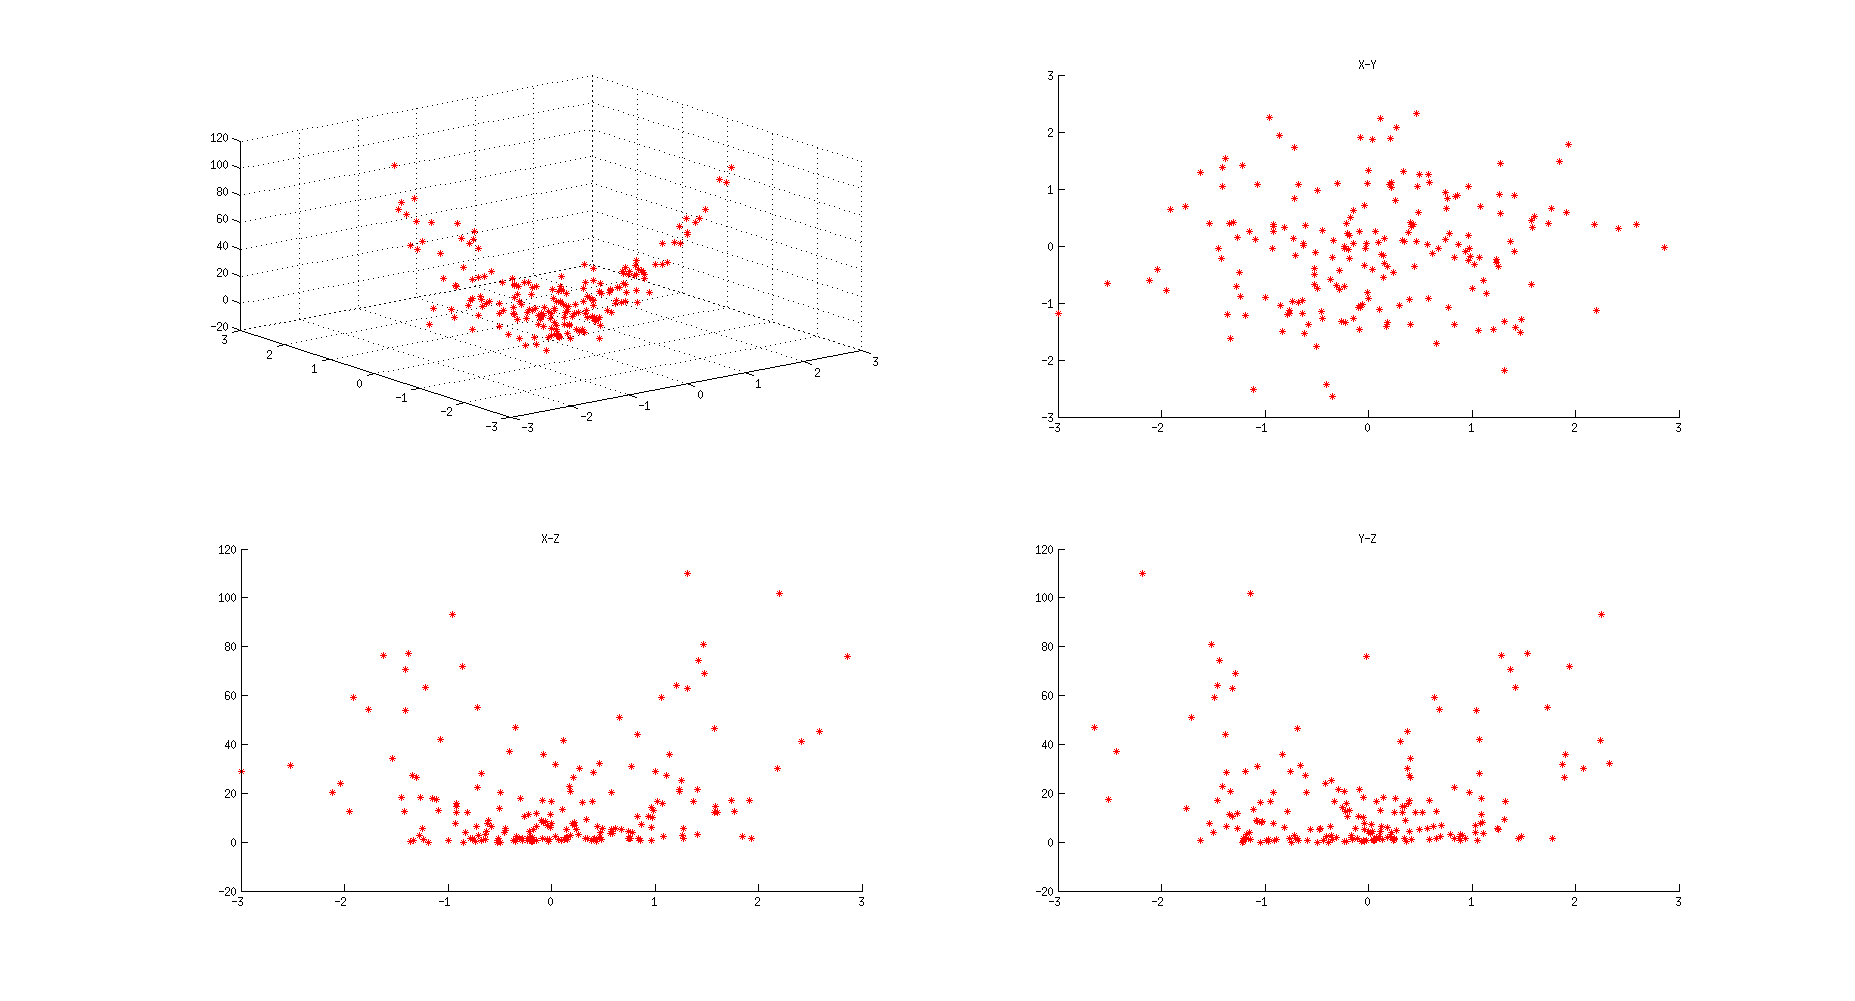
\includegraphics[width=1.00\textwidth]{figures/2-1.png}
    \caption{Graphical representation of 100 observations generated according 
        to the model given in~\ref{eq:2-1}. 2D projections on the X-Y, X-Z and 
        Y-Z planes are given for clarity.}
    \label{fig:2-1}

\end{figure}

\subsection{}
\label{subsec:2-2}

Since this is a regression problem with an 1-dimensional output $y$, a single 
output neuron was chosen, with a linear activation function. This way the output 
value $y$ is free to swing along the ranges shown in Figure~\ref{fig:2-1} and 
is not restricted to a particular interval.\vertbreak

The sigmoid function (logistic function, defined as $\frac{1}{1 + e^{x}}$) was 
chosen as the activation function for the hidden units. It seemed natural to 
include it in this 
particular case, since it is part of the model given in~\ref{eq:2-1}.\vertbreak

To include the weight decay, one followed expression 5.112 on~\cite{Bishop2006}. This 
resulted in the addition of a parcel $\lambda\textbf{w}$ when determining the 
derivatives of the error with respect to  the first-layer and second layer weights. 
A learning factor of 0.001 has been fixed. The initial set of weights are 
randomly generated within the interval [-0.5, 0.5].\vertbreak

Check the MATLAB code (and comments) in the file \verb+trainAndTestNeuralNet.m+ 
for further details.

\subsection{}
\label{subsec:2-3}

Figure~\ref{fig:2-3} shows the error curves as a function of the number of 
training epochs. A sum-of-squares error function was used of the form

\[E = \frac{1}{2}\sum_{n=1}^{N}(y_n - t_n)^2 \]

where $N$ is the number of training\slash test samples, $y_n$ is the output 
value obtained by the model after a given epoch and $t_n$ is the desired output.\vertbreak

\begin{figure}[h!]

    \centering
    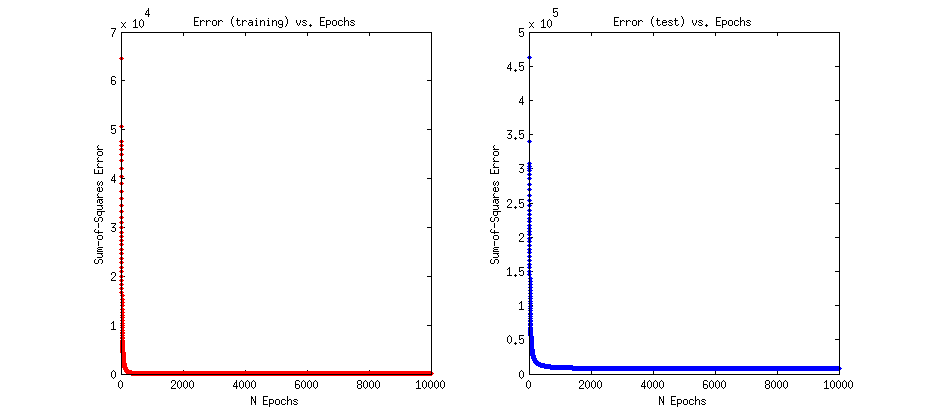
\includegraphics[width=1.00\textwidth]{figures/2-3.png}
    \caption{Training and test error curves as a function of the number of 
        training epochs, for 10000 epochs and $\lambda = 0$.}
    \label{fig:2-3}

\end{figure}

As an over-fitting behavior I was expecting to find something similar to 
that of Figure 5.12 on~\cite{Bishop2006}, in which the test error increases after 
a given number of epochs is reached. Figure~\ref{fig:2-3} shows the result 
after 10000 epochs, with a regularization factor $\lambda = 0$. By purposely not 
using a regularization factor, I have tried to force over-fitting. Such is not 
verified after 10000 epochs. In any case, the sum-of-squares error after 10000 
epochs is still large for the test error case, which indicates there's a 
problem with the implementation of the neural network.

\section{Problem 3}

\begin{table}[H]
\begin{center}
    \small
        \begin{tabularx}{0.30\textwidth}{ c | c | c }
            %\hline
            $K$     & $d(P,\hat{P} (1))$  & $(P,\hat{P} (3))$ \\ [0.5ex]
            \hline
            10    & $\infty$ & -0.326 \\ [0.5ex]
            %\hline
            20    & $\infty$ & -0.333 \\ [0.5ex]
            %\hline
            30    & $\infty$ & -0.336 \\ [0.5ex]
            %\hline
            40    & $\infty$ & -0.337 \\ [0.5ex]
            %\hline
            %\hline
        \end{tabularx}
    \caption{Results for the Kullback-Liebler divergence values for 
            $K = {10, 20, 30 40}$ and posterior calculation methods given by 
            equations (1) and (3) given in the exercise.}
    \label{tab:3-1-results}
    \end{center}
\end{table}

The results of the Kullback-Liebler divergence for equation (1) show that a 
pure KNN prediction is considered to be rather inaccurate, with a infinite 
divergence (this is caused by the values of 0 obtained for some 
$\hat{P}(C_k|x_n)$).\vertbreak

Check the MATLAB code (and comments) in the files \verb+problem3.m+, 
\verb+knnclassifier.m+ and \verb+getknn.m+ for further details.

\bibliographystyle{plain}
\bibliography{hw3.bib}

\end{document}
